\begin{mydefs}
	\begin{itemize}
	\iftoggle{eleve}{%
			\item Un nombre \hrulefill
			
			\vspace*{0.2cm}
			\hrulefill
			
			\vspace*{0.2cm}
			\hrulefill
			
			\begin{center}
				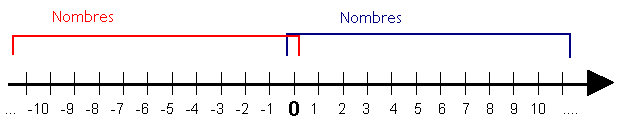
\includegraphics[scale=0.7]{relatifs_eleves}
			\end{center}
			
			\item Les nombres \hrulefill 
			
			\vspace*{0.2cm}
			\hrulefill
			
			\item Un nombre \hrulefill
			
			\vspace*{0.2cm}
			\hrulefill
			
		
			\item Deux \hrulefill
			
			\vspace*{0.2cm}
			\hrulefill
			
			\vspace*{0.2cm}
			\hrulefill
	}{%
	
		\item Un nombre supérieur à 0 est un \kw{nombre positif}, un nombre inférieur à 0 est un \kw{nombre négatif}.
		
		\begin{center}
			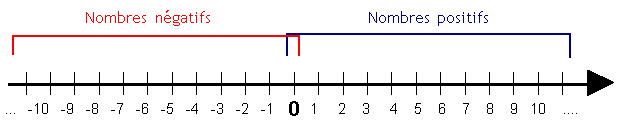
\includegraphics[scale=0.7]{relatifs}
		\end{center}
		
		\item Les nombres positifs et négatifs forment l'ensembles des \kw{nombres relatifs}.
		
		\item Un nombre relatif est composé d'\kw{un signe} (+ ou -) et d'une \kw{distance à zéro}.
		
		\item Deux \kw{nombres opposés} ont la \kw{même distance à zéro} et des \kw{signes différents} .
		
	}	
	\end{itemize}
\end{mydefs}

%\begin{myrem}
%	0 est le seul nombre à être à la fois positif et négatif.
%\end{myrem}
\newpage

\begin{myexs}
	\iftoggle{eleve}{%
		\begin{itemize}
			\item $+7$ est un nombre \hrulefill; 
			\begin{center}
				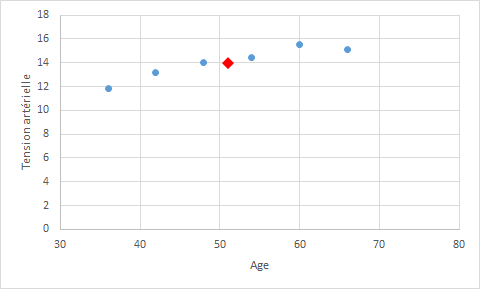
\includegraphics[scale=0.8]{ex1}
			\end{center}
			\item $\num{-4}$ est un nombre \hrulefill;
			\begin{center}
				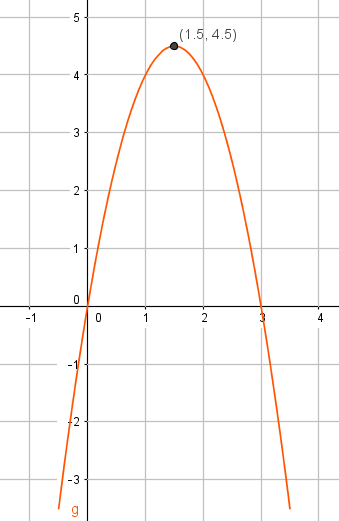
\includegraphics[scale=0.8]{ex2}
			\end{center}
			
			\item $0$ est \hrulefill %, sa distance à zéro est 0.
			\item $+10$ et $-10$ sont \hrulefill
			\begin{center}
				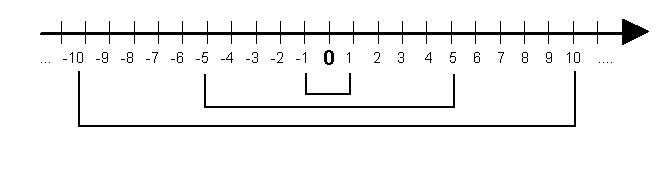
\includegraphics[scale=0.7]{opposes2}
			\end{center}
		\end{itemize}	
	}{%
	\begin{itemize}
		\item $+7$ est un nombre positif, sa distance à zéro est 7; 
		\begin{center}
			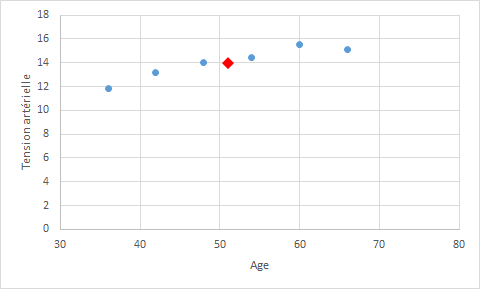
\includegraphics[scale=0.8]{ex1}
		\end{center}
		\item $\num{-4}$ est un nombre négatif, sa distance à zéro est 4;
		\begin{center}
			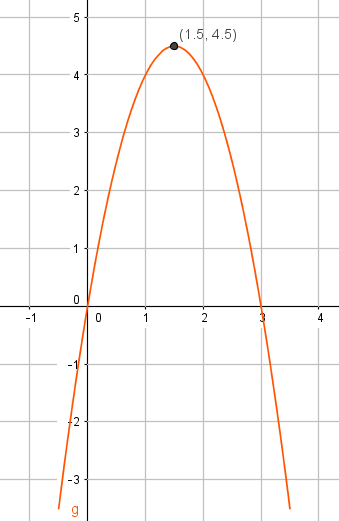
\includegraphics[scale=0.8]{ex2}
		\end{center}
	
		\item $0$ est à la fois un nombre positif et négatif.%, sa distance à zéro est 0.
		\item $+10$ et $-10$ sont des nombres opposés.
		\begin{center}
			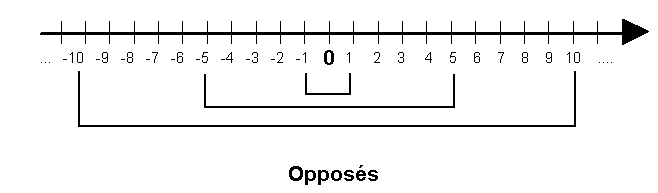
\includegraphics[scale=0.7]{opposes}
		\end{center}
	\end{itemize}
}
\end{myexs}